\documentclass[11pt, oneside]{article}   	% use "amsart" instead of "article" for AMSLaTeX format
\usepackage{geometry}                		% See geometry.pdf to learn the layout options. There are lots.
\geometry{a4paper}                   		% ... or a4paper or a5paper or ... 
%\geometry{landscape}                		% Activate for for rotated page geometry
%\usepackage[parfill]{parskip}    		% Activate to begin paragraphs with an empty line rather than an indent
\usepackage{graphicx}				% Use pdf, png, jpg, or eps§ with pdflatex; use eps in DVI mode
\usepackage{array}							% TeX will automatically convert eps --> pdf in pdflatex		
\usepackage{amssymb}
\usepackage{cite}

\title{Requirement Engineering Process in AMIDST}
\author{The handsome AMIDST guys et. al.}
\date{Latest version, \today}							% Activate to display a given date or no date

\begin{document}
\maketitle
%
%\begin{abstract}
%\end{abstract}
%
\section{Introduction}

It is widely accepted that there is a clear link between proper system requirement and project success, as described in  \cite{Boe91} and \cite{Jac99}.  Also, there is clear link between failure to understand requirements and project failure \cite{Ewu03}.  
%Although requirement engineering (RE) process is very important, the academic field is still seen as immature \cite{Poh96}. There is agreement that a definition of a requirement is related to \emph{what} a system can do and not \emph{how} it is done.  Moreover, the community acknowledge that requirements must be elicited, specified and validated.  However, the agreements seem to end there and little uniformity on terminology is reached \cite{Poh96}.  
In \cite{Ebe10} it was emphasised that since projects differ, no standard requirement engineering (RE) process exists.  In the AMIDST project, we have therefore chosen to inspect the main characteristic of the project, before choosing a paradigm for conducting the RE process.

The report is outlined as follows.  In section \ref{sec:characteristic}, the main characteristics of the process are described.  In section \ref{sec:definitions} some important definitions are discussed, while the five phases of the AMIDST RE process is outlined in section \ref{sec:reprocess}.  Throughout the paper, it is a theme that choices that are taken are argued for in relation to the characteristics identified in section \ref{sec:characteristic}.  In section \ref{sec:retrospection}, we have added a retrospection of the RE process so far.

\section{Main characteristics of the AMIDST RE process}
\label{sec:characteristic}

Prior to project start, the importance of RE was well acknowledged by the partners in the project.  This is evident from the fact that 23 out of 310 person months were assigned to conduct the requirement analysis.  We have chosen to summarise the characteristics in table \ref{tab:characteristic}, making it is easier to refer to them later in this report.

\begin{table}
\caption{Characteristics of the AMIDST RE process}
\vspace{1ex}
\begin{tabular}{
>{\raggedright\hspace{0pt}}m{8mm}%
>{\raggedright\hspace{0pt}}p{120mm}}
\hline
& \tabularnewline
1 & Some participants in the project had little experience with RE processes.  \tabularnewline
2 & The project is a consortium of 7 partners, 4 industrial and 3 universities, which are situated in 4 different countries.  This imposes a constraint on the communication channels. \tabularnewline
3 & The software is expected to be compatible with three different systems in three different domains, with three different companies. Transference of domain knowledge from the industrial partners to the academic partners is clearly a constraint in the project. \tabularnewline
4 & The software itself is based on probabilistic graphical models. It may be a challenge to educate the industrial partners on this topic, since some aspects of this topic are highly theoretical.  \tabularnewline
5 & Defining a requirement is linked with the perception of which design pattern to follow \cite{Ral13}.  A design pattern is basically the path to meet the requirement.  As explained in \cite{Ral13}, when there is a high degree of unclarity of which design design pattern to follow, this ambiguity is transferred to the definition of the requirement as well.  The goal of the AMIDST software is to reach targets that are highly innovational, meaning that it is particularly difficult to define requirements that are clear and unambiguous. \tabularnewline
6 & The RE document and the RE process itself must be in compliance with the approved application to the seventh EU programme. One challenge here is that the RE process must be finished at month seven in the project. This means that the RE process must be done in a self-contained phase, such as for instance the Waterfall process \cite{Roy70} or the V-Model \cite{For91}.  Modern software projects tend to see requirement engineering as a continuous and collateral process throughout the whole project as for instance in extreme programming \cite{Bec99}.  Generally, the Waterfall and the V-model have focus on fulfilling the needs of project management, but less on users and software developers.  This is because the real needs from users and software developers tend to evolve during a project and are difficult to state in the beginning.  It is therefore a challenge in this project that all requirements must be added before month 7.
\tabularnewline
%& \tabularnewline
\hline
\end{tabular}
\label{tab:characteristic}
\end{table}


\section{Important definitions in the AMIDST RE process}
\label{sec:definitions}

In order to meet characteristic one and two in table \ref{tab:characteristic}, we decided to bring clarity on a number of definitions that is used in the AMIDST RE process. In the next subsections we will describe what is meant by a RE process, a use case, a user group and a requirement. These definitions are necessary to fully understand the five phases of the AMIDST RE process as described in section \ref{sec:reprocess}.

\subsection{Definition of a RE process}

To date there is no common definition of RE.  Some definitions focus on elicitation of requirements and therefore the interaction with the user, while others focus on the documentation or the specification.  A definition that takes both focuses into account is the IEEE standard given in \cite{Iee90}:
\emph{
\begin{enumerate}
\item The process of studying user needs to arrive at a definition of system, hardware or software requirements.
\item The process of studying and refining system, hardware or software requirements.
\end{enumerate}
}

However, based on characteristicss two to five in table \ref{tab:characteristic}, it is clear that also representational, social and cognitive aspects need to be taken into account in the definition.   We found some comfort in a definition by \cite{Lou95}:

\emph{A systematic process of developing requirements through an iterative co-operative process of analysing the problem, documenting the resulting observations in a variety of representation formats and checking the accuracy of the understanding gained.}

\subsection{Definition of a user group}

Within each organisation we decided to group the users into a small set of user groups. The users within each user group  have similar roles within their organisation and their set of competences are expected to be similar. This is essential to meet characteristics three in table \ref{tab:characteristic}.  Also, the user groups play a central role in how to write the use cases, which is the topic of the next definition.

\subsection{Definition of a use case}

In software and systems engineering, a use case is a list of steps, typically defining interactions between an actor and a system, to achieve a goal. The actor can be a human or an external system \cite{Poh10}.  An overview on how to write effective use cases is given in \cite{Coc01}, where several templates are given.  In the AMIDST project, we have decided to keep a simple definition to meet characteristics one. The use case providers are asked to provide the use cases in natural language and for each use case the following questions are central:

\begin{enumerate}
\item Who are the actors involved in the use case? An actor is either a person belonging to a user group or an entity that interacts with the AMIDST framework.  
\item What is the main event that initiates the use case? This could e.g. be an external business event or a system event that causes the use case to begin.  It could also be the initial step in a normal work flow. 
\item What are the main user actions and system responses that will take place during the normal execution of the use case?. This dialog sequence will ultimately lead to accomplishing the goal that is implied by the use case name and description.
\item How can we evaluate the success of the use case?
\end{enumerate}

\subsection{Definition of a requirement}

It is also of important to give clarity the definition of a requirement in the AMIDST project.  The IEEE standard is given in \cite{Iee90}: 
\emph{
\begin{enumerate}
\item A condition or capability needed by a user to solve a problem or achieve an objective. 
\item A condition or capability that must be met or possessed by a system or system component to satisfy a contract, standard, specification or other formally imposed document. 
\item A documented representation of a condition or capability as in 1 or 2.
\end{enumerate}
}

This definition has a clear focus on the user, the system/system component and also which contract, standard or specification is needed to be met.  This is particularly tractable in the AMIDST project where most contributors understand only parts of the project, as understood by characteristics 3 and 4 in table \ref{tab:characteristic}. Notice, that this definition does not allow for a requirement to be to some degree optional,.  This is needed to meet characteristics 5 in table \ref{tab:characteristic} and as an extension we introduce the term \emph{optional requirements}. The term optional requirement is used when the system is required to meet only a fraction of the optional requirements.  The requirements are divided up into three categories; must, should and could, which clarifies how \emph{optional} they are.

A requirement is also associated with a step in a product life cycle as described and \cite{Eig09}.  In this reference the overall life cycle is divided into three phases; design phase, operation phase and disposal phase.  In the AMIDST project we only considered the two first phases and figure \ref{REprocess2} shows the AMIDST product life cycle.

\begin{figure}
\centering
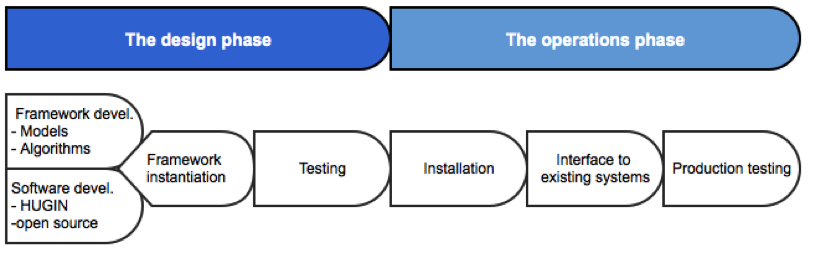
\includegraphics [keepaspectratio,width = 14cm] {REprocess2}
\caption{The table show key steps in the design and operation stages. Notice that each requirement can only be member of one step.}
\label{REprocess2}
\end{figure}

The design stage contains general functionality requirements for the system, i.e. what the system should do and support.  In figure \ref{REprocess2}, we detail key steps inside this phase. The first step consists of the design of the general framework (models and algorithms) as well as the design and development of the software tools. In a second step, the general framework and software is instantiated for each specific use case. Finally, initial tests of the use case instantiated framework are conducted.  At the design phase, possible design requirements could e.g. address
\begin{itemize}
 \item the scope of the model
 \item the interpretability of the learned models
 \item the extent and type of domain knowledge that can be integrated into the models
 \item documentation
\end{itemize}

The requirements for the operation phase concern the functionality of the deployed system. In figure \ref{REprocess2}, we decompose this phase into three stages: installation, interface to existing systems, and production testing. The requirements for this phase could e.g. address
\begin{itemize}
 \item hardware constraints
 \item interfaces to existing software or data base systems
 \item inference functionality, i.e., what queries the system should be able to answer
\end{itemize}

In the AMIDST process all requirements are associated with only one of these steps to meet characteristics three in table  \ref{tab:characteristic}.  Moreover, the requirements are also associated with work package and task numbers to meet characteristics two in table \ref{tab:characteristic}.

\section{The five phases of AMIDST RE process}
\label{sec:reprocess}

The overall RE process is carried out in an iterative fashion that is expected to involve a high level of cooperation and interaction between the partners in order to meet all characteristic in table \ref{tab:characteristic}. During this process the document for the requirements analysis will be gradually refined and expanded. In figure \ref{REprocess1}  an illustration of the RE process for AMIDST is given, which is inspired by \cite{Ebe10}.  In general the process contain five phases, which are discussed below.
\begin{enumerate}
 \item Preparation I.  This phase started with Work Package 1 and ended when the initial template for the RE document was finished.  This template can be found in attachment X1. In this template there is emphasis on a number of definitions in RE to meet characteristics one in table \ref{tab:characteristic}.  Moreover, the use case providers are asked to provide a detailed description of the system context that the AMIDST software is expected to run in, identify which user groups are involved and finally describe use cases and requirements.  These actions are in compliance with characteristics three in table \ref{tab:characteristic}.  
\item Elicitation. The distribution of the above mentioned template marks the initialisation of this phase.  Its aim is to get an initial high-level description of the different use cases and their requirements. This information are specified by the use case providers in collaboration with the academic partners to meet characteristics four and also five and six in table \ref{tab:characteristic}.  Once the use case providers return the present document with the requested information, feedback and informal meetings are expected to clarify and refine the information provided.  At the end of the elicitation phase, the aim is to have a first coherent description of the requirements for each use case provider.
 \item Prioritization. In this phase the use case providers completes an extended version of the document template used in the previous phase. This template is used to link each of the requirements to the relevant work packages and tasks in the AMIDST project. Moreover, the template allows the use case providers to provide a more fine grained prioritization of the relevant requirements for the AMIDST framework.  Specifically, the use case providers are asked to rate each requirement in terms of how important it is to them.  In this step it is of key importance to ensure that characteristics 7 in table  \ref{tab:characteristic} is met.
 \item Validation. In this phase, the requirements from all use-case providers are collected to get the \emph{big picture}.  This involves a discussion to what extent the requirements can be accommodated. Revisions and negotiations of the detailed requirements are therefore expected.  
 \item Evaluation and Testing. In this phase, the focus is on the elicitation of the evaluation and testing procedures in the AMIDST project. This phase starts with the distribution of a new document template, where the aim is to obtain a high level description of the evaluation and testing methods that is necessary to measure the performance of the AMIDST framework.
\end{enumerate}

\begin{figure}
\centering
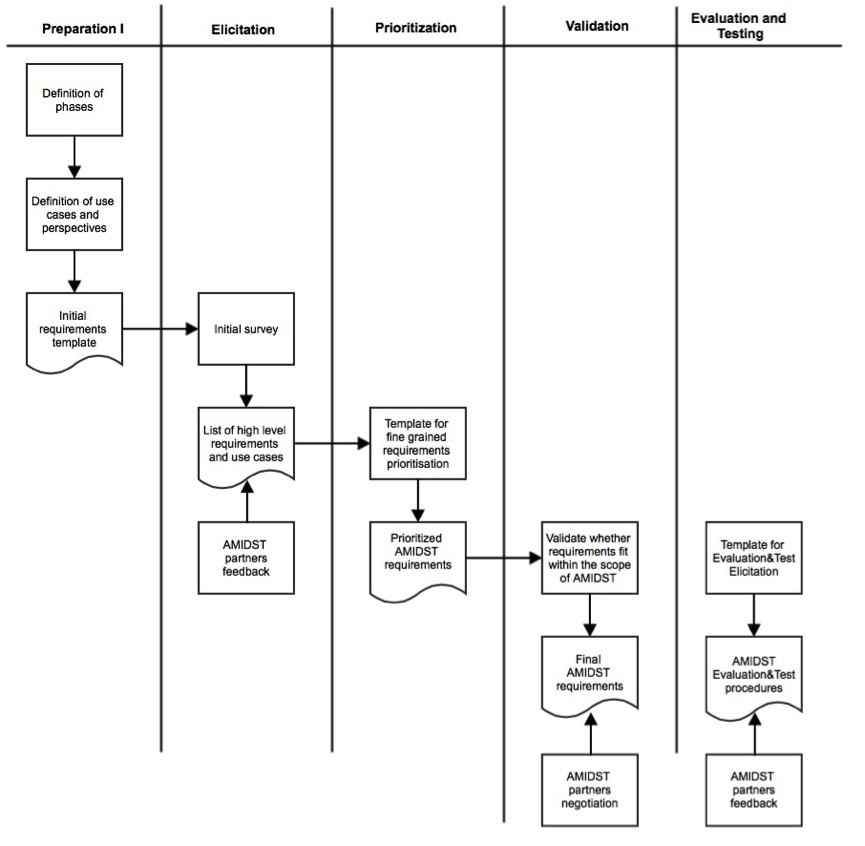
\includegraphics [keepaspectratio,width = 14cm] {REprocess1}
\caption{Description of the five phases in the RE process in AMIDST.}
\label{REprocess1}
\end{figure}

\subsection{Additional comments to AMIDST the RE process}

It is appropriate to make a few comments related to characteristics two in table \ref{tab:characteristic} and also the need for massive knowledge transfer in the project.  No constraints on the form of the meetings are set.  Communication is done through meetings, video calls, telephone, email and document transferral.  The participants in the meetings could range from a large group to only a few people.  The reason for the \emph{no constraint policy} is to encourage as much knowledge transfer as possible.  The formal parts are taken into account in the RE documents that will be delivered at the end of the RE process. 

\section{Retrospection of the process so far}
\label{sec:retrospection}

This part of the report is written in month six when most of the process is conducted.  This section contains a few points on what experiences we have gained in the project so far

Some important experiences in this project have been:

\begin{enumerate}
\item Everyone involved has had a learning experience on many levels.  The industrial partners have learned about probabilistic graphical models, while the academic partners have learned about the industrial domains.  Most participants have increased their knowledge on how to conduct a requirement analysis. 
\item There has only been one meeting where all stakeholders have met, which was the kickoff meeting in Denmark in month three.  Most communication has been done through Skype and email, but also a few face to face meetings have taken place. Most of the communications have been related to clarifications in terms of filling out the template X1.
\item There have been adjustments of the template X1 as the process has proceeded.  Examples of this is adding fields to the requirements so they could be linked to concrete tasks in the AMIDST project or adding columns for rating the importance of a requirement.
\end{enumerate}



\bibliographystyle{splncs}
\bibliography{re}


\end{document}  